\chapter{RESULTS}
\label{chap:results}

% By labeling the chapter, I can refer to it later using the
% label. (\ref{chap:intro}, \pageref{chap:intro}) Latex will take care
% of the numbering.
There are two classes of results discussed here: ground state energy convergence
and excitation spectra of atomic nuclei. Existing interacting shell
model codes such as BIGSTICK have errors with respect to experiment of around
a few hundred keV. Since our interacting shell model PNISM is an approximation to these results
found in BIGSTICK, and are bounded by the variational principle (see Appendix \ref{VP}),
we expect the results computed by PNISM to converge to the results of BIGSTICK
as the size of the basis is increase. Ground state energies are found to 
converge exponentially and monotonically with the size of the basis, and excitation 
spectra also converge to the results of BIGSTICK, although in a more sporadic
and unpredictable way. This is because PNISM is a J-scheme code: we should expect
that the excitation spectra for fixed-J to obey the variational principle, but a
plot of low-lying excitations, having mixed J-values, will have non-monotonic
convergence curves. This can be understood by realizing that as each fixed-J
excitation spectra settles downward towards the energy of the untruncated basis, 
the gaps between ordered energy levels may grow or shrink as excitation spectra from different 
J values converge at different rates. This can be seen in the excitation plots at
the end of the chapter. 

Results demonstrate the exponential convergence of the ground 
state energy as a function of the number of states retained, for nuclei 
where a full diagonalization is possible even on a laptop. Results are given
for sample nuclei in both the sd shell and the pf shell. When all of the states
are retained, the results are exactly equal to those of BIGSTICK.
Results also demonstrate the convergence of low-lying excitations in the
sd and pf shells. When all of the states are retained, the results are exactly 
equal to those of BIGSTICK for all excitation levels. Qualitatively one can observe that $N>Z$ nuclei tend
to converge faster than $N=Z$ nuclei.

In order to examine the convergence of the wavefunctions, we calculated
the density matrices for nuclei in both model spaces. As expected, when all 
of the states are included, the results converge to those of BIGSTICK. 

\section{Capstone Calculations}
These calculations are meant to push PNISM to its limits to demonstrate its use.
We study three nuclei, $^{56}$Ni, $^{60}$Ni and $^{64}$Ge in the ($p_{1/2}$, $p_{3/2}$, $f_{5/2}$, $f_{7/2}$) 
model space. The M-scheme basis dimensions
of these nuclei are compared in Table \ref{mschemecap}.
The M-scheme dimensions of the proton Hamiltonian and the neutron Hamiltonian for
these nuclei is shown in Table \ref{jschemecap}. 
(These are used
by PNISM to build the J-scheme basis for nuclei in the ($p_{1/2}$, $p_{3/2}$, $f_{5/2}$, $f_{7/2}$) model
space.)

\begin{table}[h]
    \caption{M-scheme Dimensions for Select Nuclei in the ($p_{1/2}$, $p_{3/2}$, $f_{5/2}$, $f_{7/2}$) \hspace{\textwidth}Model
Space}
    \label{mschemecap}
%\centering
\begin{tabular}
    {c c c c c c c c}
    \hline 
    \hline
Nuclide & Val. protons & Val. neutrons & M-scheme dim. & Ground state E [MeV] \\
$^{56}$Ni & 8 & 8 &   $1.09\times 10^9$ & -72.56190 \\  
$^{60}$Ni & 8 & 12 &  $1.09\times 10^9$ & -80.26105\\
$^{64}$Ge & 12 & 12 & $1.09\times 10^9$ & -98.81734\\
    \hline
    \hline
\end{tabular}
\end{table}
\begin{table}[h]
    \caption{Dimensions for Proton and Neutron Hamiltonians}
    \label{jschemecap}
%\centering
\begin{tabular}
    {c c c c c c c c}
    \hline 
    \hline
Hamiltonian & Val. protons & Val. neutrons & M-scheme dim. \\
$\hat{H}_{neutron}$ & 0 & 8 &  12022 \\
$\hat{H}_{proton}$ & 8 & 0 &  12022 \\
$\hat{H}_{proton}$ & 12 & 0 & 12022 \\
$\hat{H}_{neutron}$ & 0 & 12 & 12022 \\
    \hline
    \hline
\end{tabular}
\end{table}

When 
computing the excitation spectra of these nuclei and limiting ourselves to $16$ GB of memory, we were able
to keep up to $200$ of the $12022$ available eigenstates of the pure proton and
pure neutron Hamiltonians.  
Exact dimensions of the truncated J-scheme basis are given for $^{56}$Ni in Table \ref{56nit}.
(As a function of number $N$ of proton and neutron wavefunctions retained
for coupled J-scheme basis using M-scheme solutions in the ($p_{1/2}$, $p_{3/2}$, $f_{5/2}$, $f_{7/2}$) model
space. $N_{max}=12022$. J-scheme dimension is the size of the Hamiltonian for fixed $J$. Absolute error and
percent error are computed relative to M-scheme solution from BIGSTICK.)
The same data for $^{60}$Ni is found in Table \ref{60nit}. 
(As a function of number $N$ of proton and neutron wavefunctions retained
for coupled J-scheme basis using M-scheme solutions in the ($p_{1/2}$, $p_{3/2}$, $f_{5/2}$, $f_{7/2}$) model
space. $N_{max}=12022$. J-scheme dimension is the size of the Hamiltonian for fixed $J$. Absolute error and
percent error are computed relative to M-scheme solution from BIGSTICK.)
Computing the matrix elements of the Hamiltonian for a calculation of a handful low-lying states
requires several sets of bases for different $J$ values. 

\begin{table}[h]
    \caption{$^{56}$Ni Ground State Energy and J-scheme Dimensions}
    \label{56nit}
%\centering
\begin{tabular}
    {c c c c c c c c}
    \hline 
    \hline
$N$ & J-scheme dim. & Ground state E [MeV] & Abs. error & Perct. error \\
10  &22    &   -70.558 & 2.004  & 2.76 \\
50  &384   &   -71.957 & 0.6049 & 0.833\\
100 &1408  &   -72.010 & 0.5519 & 0.761\\
200 &5128  &   -72.195 & 0.3669 & 0.506\\
400 &19838 &   -72.318 & 0.2439 & 0.336\\
600 &43912 &   -72.424 & 0.1383 & 0.191\\
    \hline
    \hline
\end{tabular}
\end{table}
\begin{table}[h]
    \caption{$^{60}$Ni Ground State Energy and J-scheme Dimensions}
    \label{60nit}
%\centering
\begin{tabular}
    {c c c c c c c c}
    \hline 
    \hline
$N$ & J-scheme dim.   & Ground state E [MeV] & Abs. error & Perct. error \\
10  & 20    & -76.731 & 3.5400 & 4.398 \\
50  & 412   & -78.839 & 1.4221& 1.778 \\
100 & 1477  & -79.000 & 1.2611& 1.571 \\
200 & 5424  & -79.408 & 0.8531& 1.063 \\
400 & 20459 & -79.869 & 0.3921& 0.4885 \\
600 & 45086 & -80.046 & 0.2151& 0.2679 \\
    \hline
    \hline
\end{tabular}
\end{table}


\section{Heavy Nuclei}
In the future we would like to target a number of specific nuclei relevant to 
important experimental physics. In this section I will provide estimates for the 
dimension of these problems in the M-scheme, and the dimensions of the proton
and neutron Hamiltonians that would need to be solved in their place in order
to construct the J-scheme basis.

Some experimental searches for non-baryonic dark matter involve collisions
with heavy nuclei such as $^{131}$Xe, and require detailed nuclear structure calculations\cite{Bednyakov}.
Xe isotopes, as well as the Cs isotopes for studying the nuclear anapole moment,
can both be computed in the model space with single particle orbits:
\begin{equation}\label{gcn5082}
    g_{7/2},\ d_{5/2},\ d_{3/2},\ s_{1/2},\ h_{11/2},
\end{equation}
which will be referred to as the GCN5082 model space, after the name of the interaction
file used for this configuration space.
The M-scheme dimension of $^{133}$Cs and $^{131}$Xe are both around $1.98 \times 10^8$.
$^{131}$Xe has $77$ neutrons and $54$ protons, while $^{133}$Cs has $78$ neutrons
and $55$ protons. The fact that these both have an unequal number of protons 
and neutrons is encouraging; our J-scheme approximation is predicted to be 
well suited for such nuclei.


The origin of the matter-antimatter symmetry 
violation may be due to CP-violation\cite{Sakhorav}, and one approach to investigating the 
source of CP-violation is through the permanent electric dipole moments of certain
nuclei such as $^{199}$Hg\cite{Willmann}. Model spaces for nuclei with such a high
mass number do not yet exist, and we would have to create the interaction
for it. Nonetheless we can still predict the M-scheme dimensions of the proton and
the neutron parts of the Hamiltonian. $^{199}$Hg has $80$ protons and $119$ neutrons.
This means that the proton Hamiltonian will most likely be computed in the
GCN5082 model space (see equation (\ref{gcn5082}), and the neutron Hamiltonian
would have to be computed in a new shell model space. This could be defined
by the set of orbitals
\begin{equation}\label{newspo}
   1h_{9/2},\ 2f_{7/2},\ 2f_{5/2},\ 3p_{3/2},\ 3p_{1/2},\ 1i_{13/2},
\end{equation}
which corresponds to between $82$ and $126$ nucleons. (The next pair of consecutive magic 
numbers.) 

Table \ref{estimates} contains estimates for the M-scheme dimension of the Hamiltonian
for these nuclei of interest. It also provides estimates for the M-scheme dimension of the
proton Hamiltonian and the neutron Hamiltonian that would need to be solved in order
to compute the J-scheme basis for PNISM. These are orders of magnitude smaller than 
the full interaction's dimension. The estimted dimension of the M-scheme
 proton Hamiltonian for $^{199}$Hg corresponds to a calculation in the GCN5082 space, while the 
neutron Hamiltonian is estimated for the new single-particle space defined by (\ref{newspo}).

\begin{table}[h]
    \caption{Estimated Dimensions of Target Heavy Nuclei.}
    \label{estimates}
    \begin{tabular}
        {c c c c c}
        \hline
        \hline
        Nucleus    & Space   & M-scheme dim.      & Proton dim. & Neutron dim. \\
        $^{133}$Cs & GCN5082 & $1.98 \times 10^8$ & $1500$ & $7500$ \\
        $^{131}$Xe & GCN5082 & $1.98 \times 10^8$ & $1500$ & $7500$ \\
        $^{199}$Hg & Unknown & Unknown            & $36$   & $1.04\times 10^6$\\
        
        \hline
        \hline
    \end{tabular}

\end{table}


\begin{figure}
    \centering
    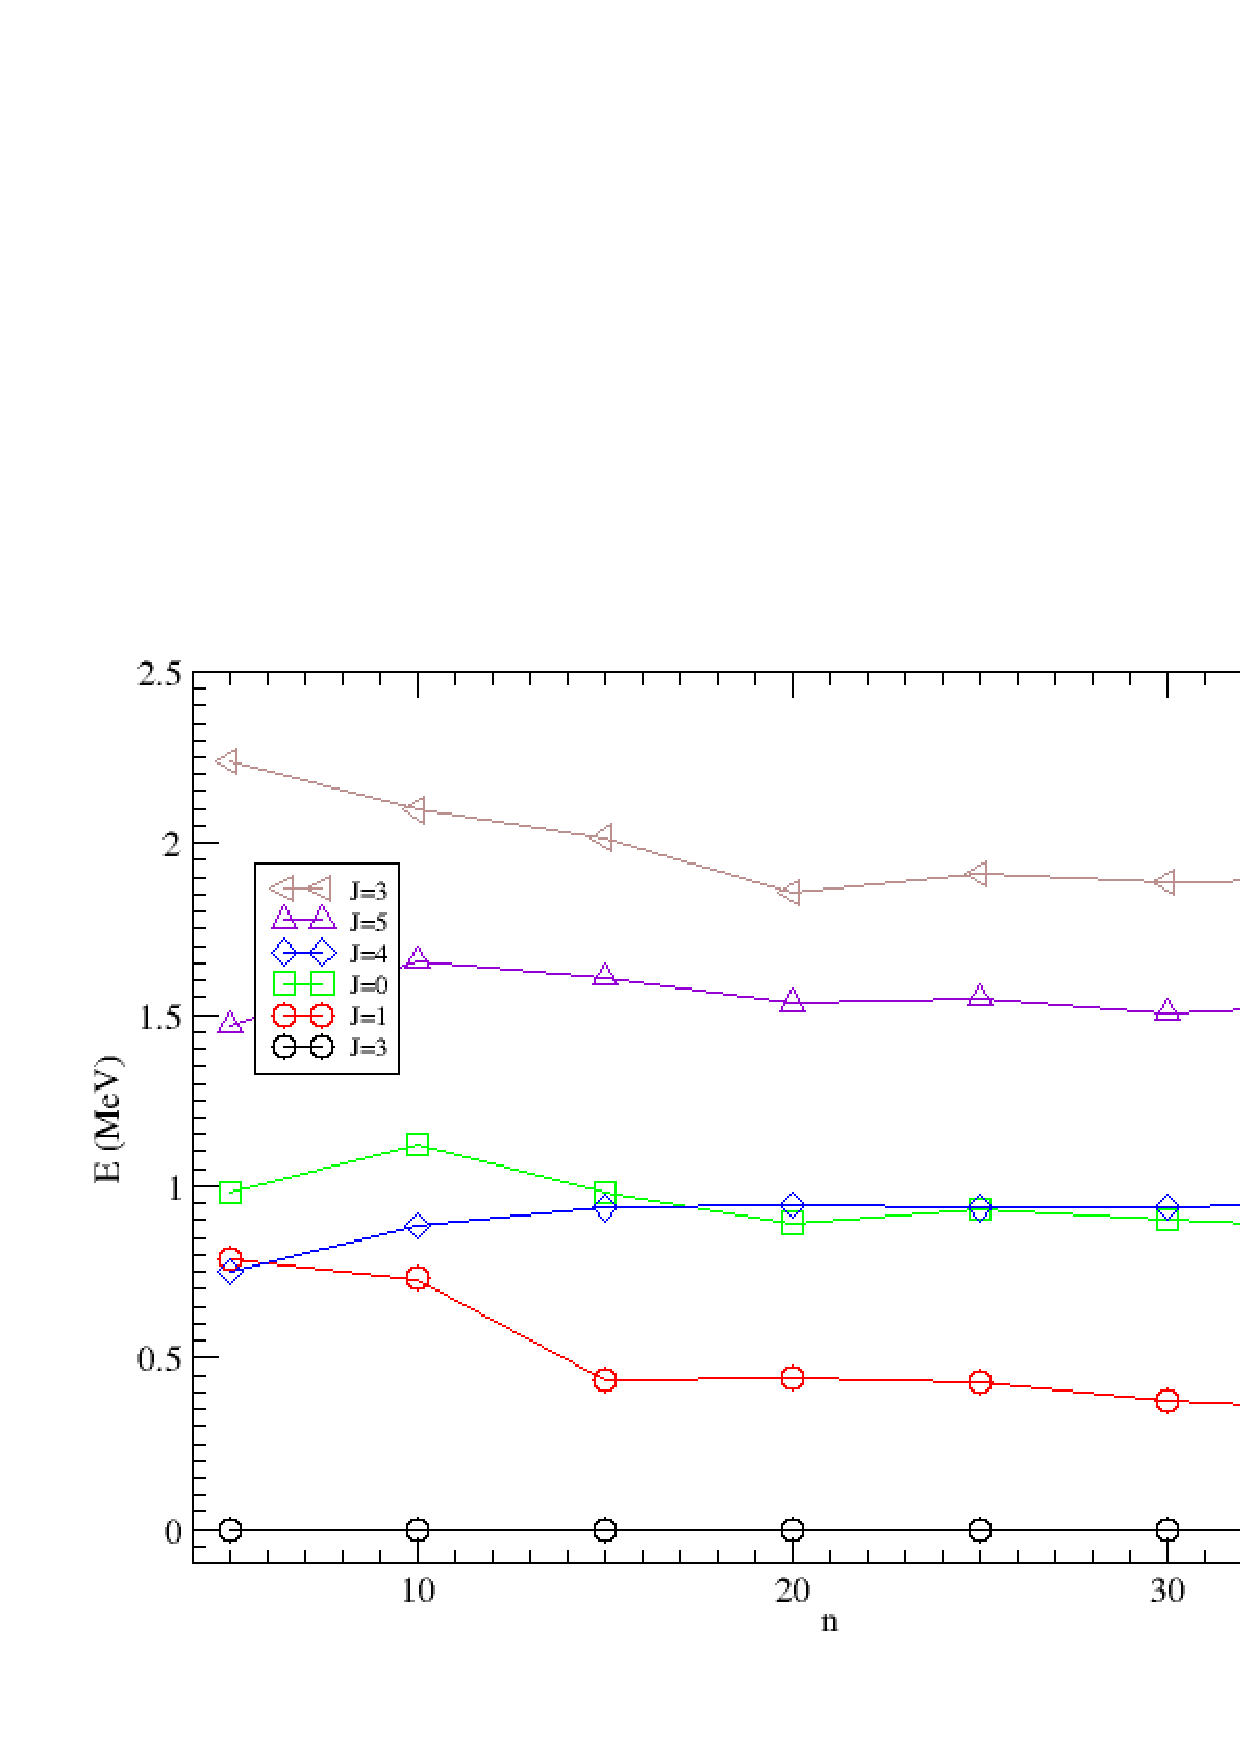
\includegraphics[width=.75\textwidth,clip]{Figures/pnism_ex_22na}
    \caption{$^{22}$Na low-lying excitation spectra as a function of $n$, the number of eigenstates retained from the pure proton and pure neutron
interactions used to form the basis. Here the maximum value of $n$ is $n=37$, when the entire basis is retained.}
    \label{22na}
\end{figure}
\begin{figure}
    \centering
    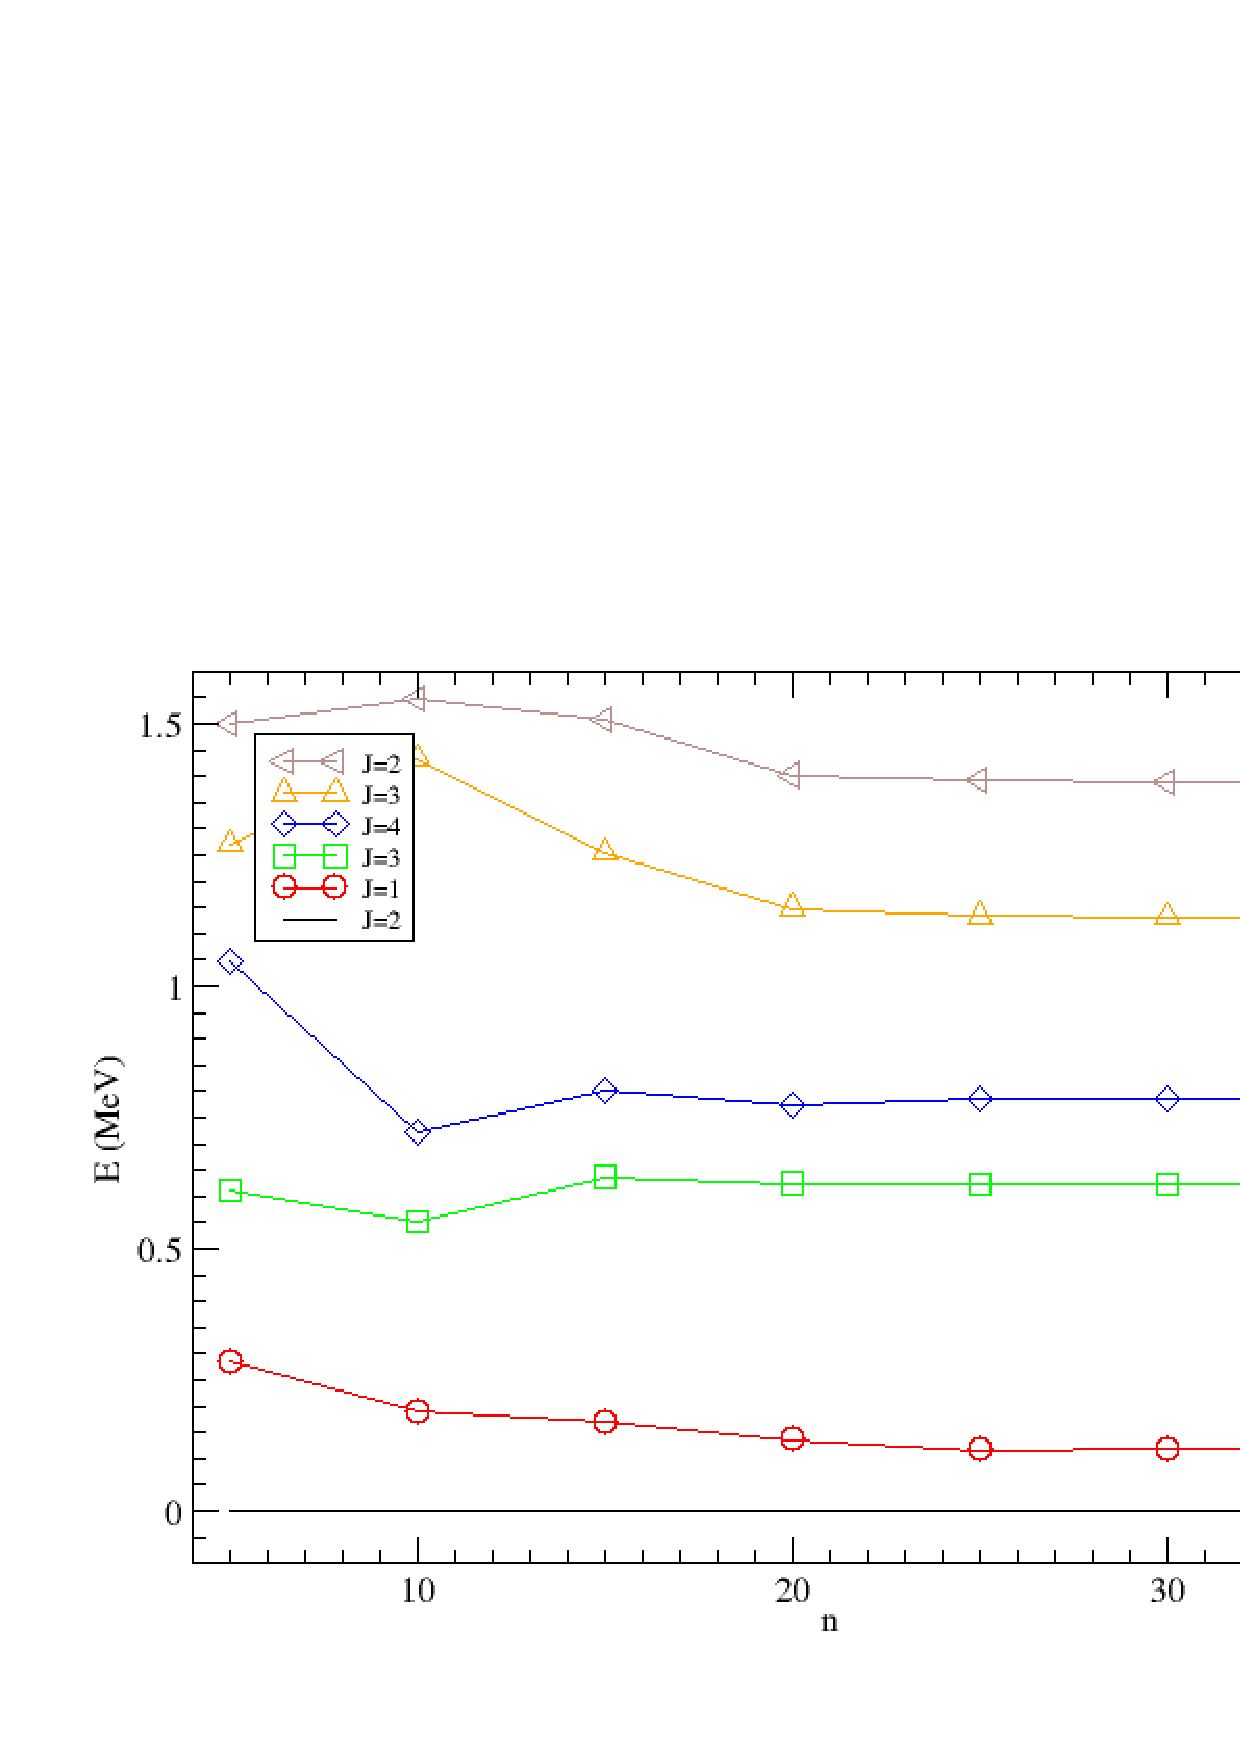
\includegraphics[width=.75\textwidth,clip]{Figures/pnism_ex_28na}
    \caption{$^{28}$Na low-lying excitation spectra as a function of the number of retained $n$. \boldmath$n_{max}=37$. Notice that $^{28}$Na
    converges faster than $^{22}$Na, while having the same basis dimensions.}
\end{figure}
\begin{figure}
    \centering
    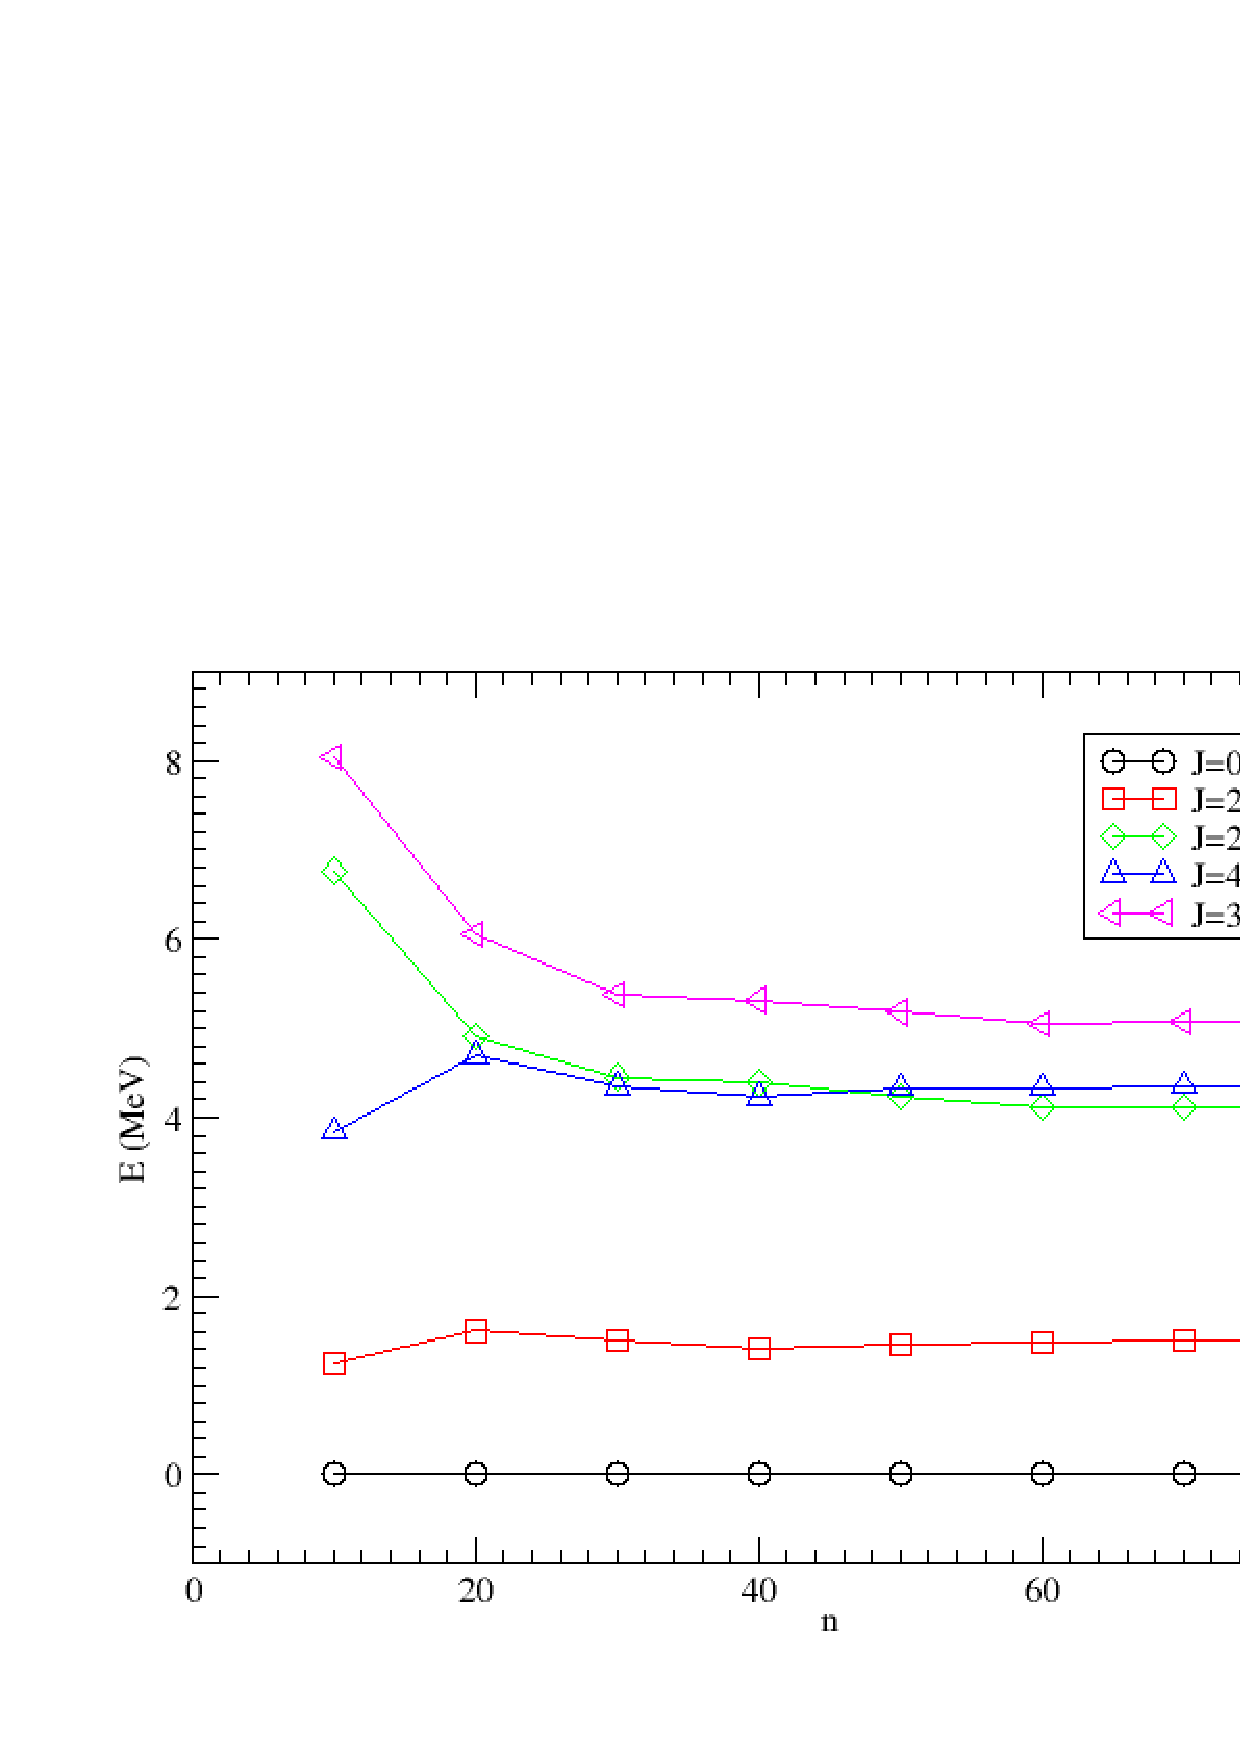
\includegraphics[width=.75\textwidth,clip]{Figures/pnism_ex_24mg}
    \caption{$^{24}$Mg low-lying excitation spectra. Symbols as in Figure \ref{22na}. Here \boldmath$n_{max}=81$.}
\end{figure}
\begin{figure}
    \centering
    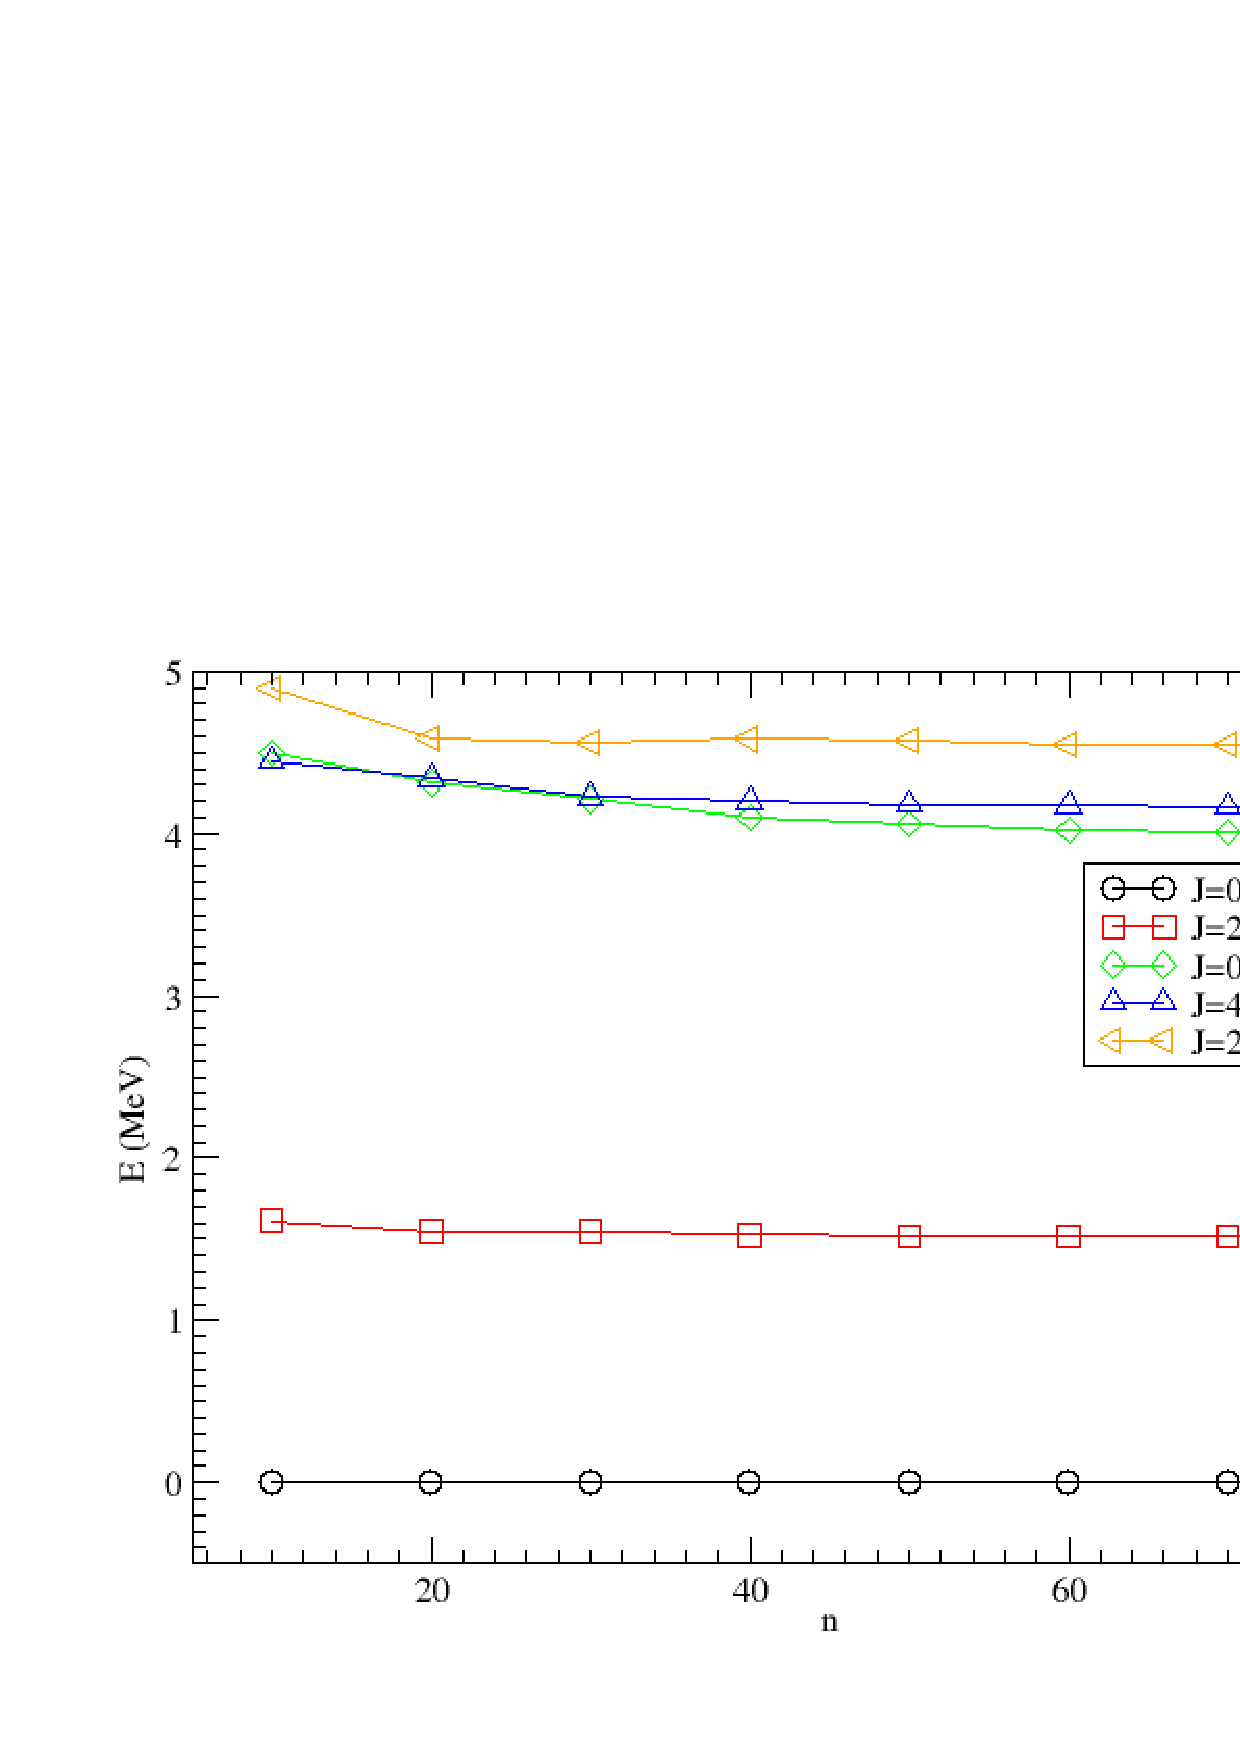
\includegraphics[width=.75\textwidth,clip]{Figures/pnism_ex_28mg}
    \caption{$^{28}$Mg low-lying excitation spectra. Symbols as in Figure \ref{22na}. \boldmath$n_{max}=81$ is the same as for $^{24}$Mg,
    but energies converge faster for $^{28}$Mg.}
\end{figure}
\begin{figure}
    \centering
    \includegraphics[width=.75\textwidth,clip]{Figures/E0_Ni56}
    \caption{$^{56}$Ni ground state energy convergence relative to complete basis wavefunction. }
\end{figure}
\begin{figure}
    \centering
    \includegraphics[width=.75\textwidth,clip]{Figures/Ni56}
    \caption{$^{56}$Ni low-lying excitation spectra. Unmarked curves are results from M-scheme calculation.}
\end{figure}
\begin{figure}
    \centering
    \includegraphics[width=.75\textwidth,clip]{Figures/E0_Ni60}
    \caption{$^{60}$Ni ground state energy convergence relative to complete basis wavefunctions as a function of the number of single-species basis states retained.}
\end{figure}
\begin{figure}
    \centering
    \includegraphics[width=.75\textwidth,clip]{Figures/Ni60}
    \caption{$^{60}$Ni low-lying excitation spectra. Unmarked curves are results from M-scheme.}
\end{figure}






